
\documentclass{sigplanconf}

% The following \documentclass options may be useful:

% preprint      Remove this option only once the paper is in final form.
% 10pt          To set in 10-point type instead of 9-point.
% 11pt          To set in 11-point type instead of 9-point.
% authoryear    To obtain author/year citation style instead of numeric.
\synctex=-1

\usepackage[utf8]{inputenc}
\usepackage{array}
\usepackage{color}
\usepackage{amsmath}
\usepackage{amssymb}
\usepackage{fixltx2e}
\usepackage{graphicx}
\usepackage[unicode=true,pdfusetitle,
 bookmarks=true,bookmarksnumbered=false,bookmarksopen=false,
 breaklinks=false,pdfborder={0 0 1},backref=false,colorlinks=false]{hyperref}


\makeatletter
\usepackage{enumitem}
\usepackage{multicol}

% nice listings
\usepackage{xcolor}
\usepackage{newverbs}

\usepackage{color}
\definecolor{verylightgray}{rgb}{0.93,0.93,0.93}
\definecolor{darkblue}{rgb}{0.2,0.2,0.6}
\definecolor{commentgreen}{rgb}{0.25,0.5,0.37}
\usepackage{letltxmacro}

\usepackage{listings}

\makeatletter
\LetLtxMacro{\oldlstinline}{\lstinline}

\renewcommand\lstinline[1][]{%
  \Collectverb{\@@myverb}%
}

\def\@@myverb#1{%
    \begingroup
    \fboxsep=0.2em
    \colorbox{verylightgray}{\oldlstinline|#1|}%
    \endgroup
}
\makeatother




\lstset{backgroundcolor={\color{verylightgray}},
  basicstyle={\scriptsize\ttfamily},
  commentstyle={\ttfamily\color{commentgreen}},
  keywordstyle={\bfseries\color{darkblue}},
  morecomment={[l]{//}},
  tabsize=4,
  morekeywords={foreach,in,def,type,dynamic,Int,
    Boolean,infer,void,super,if,boolean,int,else,
    while,do,extends,class,assert,for,switch,case,
    private,protected,public,const,final,static,
    interface,new,true,false,null,return}}
\renewcommand{\lstlistingname}{Listing}



\newcommand{\mynote}[2]{%
  \textcolor{red}{%
    \fbox{\bfseries\sffamily\scriptsize#1}%
    {\small$\blacktriangleright$\textsf{\emph{#2}}$\blacktriangleleft$}%
  }%
}

\newcommand\remi[1]{\mynote{Remi}{#1}}
\newcommand\cfbolz[1]{\mynote{cfbolz}{#1}}
\newcommand\arigo[1]{\mynote{arigo}{#1}}



\begin{document}

\special{papersize=8.5in,11in}
\setlength{\pdfpageheight}{\paperheight}
\setlength{\pdfpagewidth}{\paperwidth}

\conferenceinfo{ICOOOLPS workshop 2014}{July 28th, 2014, Uppsala, Sweden}
\copyrightyear{2014}
%\copyrightdata{978-1-nnnn-nnnn-n/yy/mm}
\doi{nnnnnnn.nnnnnnn}

% Uncomment one of the following two, if you are not going for the
% traditional copyright transfer agreement.

%\exclusivelicense                % ACM gets exclusive license to publish,
                                  % you retain copyright

%\permissiontopublish             % ACM gets nonexclusive license to publish
                                  % (paid open-access papers,
                                  % short abstracts)

%% \titlebanner{banner above paper title}        % These are ignored unless
%% \preprintfooter{short description of paper}   % 'preprint' option specified.

\title{Virtual Memory Assisted Transactional Memory for Dynamic Languages}
\subtitle{DLS'14}

\authorinfo{Remigius Meier}
           {Department of Computer Science\\ ETH Zürich}
           {remi.meier@inf.ethz.ch}
\authorinfo{Armin Rigo}
           {www.pypy.org}
           {arigo@tunes.org}

\maketitle

\begin{abstract}
....
\end{abstract}

%\category{CR-number}{subcategory}{third-level}

% general terms are not compulsory anymore,
% you may leave them out
%% \terms
%% term1, term2

\keywords
...

\section{Introduction}


Dynamic languages like Python, PHP, Ruby, and JavaScript are usually
regarded as very expressive but also very slow. In recent years, the
introduction of just-in-time compilers (JIT) for these languages (e.g.
PyPy, V8, Tracemonkey) started to change this perception by delivering
good performance that enables new applications. However, a parallel
programming model was not part of the design of those languages. Thus,
the reference implementations of e.g. Python and Ruby use a single,
global interpreter lock (GIL) to serialise the execution of code in
threads.

While this GIL prevents any parallelism from occurring, it also
provides some useful guarantees. Since this lock is always acquired
while executing bytecode instructions and it may only be released
in-between such instructions, it provides perfect isolation and
atomicity between multiple threads for a series of
instructions. Another technology that can provide the same guarantees
is transactional memory (TM). \remi{cite our position paper}

There have been several attempts at replacing the GIL with TM. Using
transactions to enclose multiple bytecode instructions, we can get the
very same semantics as the GIL while possibly executing several
transactions in parallel. Furthermore, by exposing these
interpreter-level transactions to the application in the form of
\emph{atomic blocks}, we give dynamic languages a new synchronisation
mechanism that avoids several of the problems of locks as they are
used now.

\remi{cite and extract from (our pos. paper):}
TM systems come in can be broadly categorised as hardware based (HTM),
software based (STM), or hybrid systems (HyTM). HTM systems are limited
by hardware constraints, while STM systems have a lot of overhead.
In this paper, we describe how we manage to lower the overhead of our
STM system so that it can be seen as a viable replacement for the GIL.

Our contributions include:
\begin{itemize}[noitemsep]
\item We introduce a new software transactional memory (STM) system
  that performs well even on low numbers of CPUs. It uses a novel
  combination of hardware features\arigo{"OS-level feature" maybe.
  "Hardware feature" implies it only works on custom chips}
  and garbage collector (GC)
  integration in order to keep the overhead of STM very low.
\item This new STM system is used to replace the GIL in Python and is
  then evaluated extensively.
\item We introduce atomic blocks to the Python language to provide a
  backwards compatible, composable synchronisation mechanism for
  threads.
\end{itemize}



\section{Background}


\subsection{Transactional Memory}

Transactional memory (TM) is a concurrency control mechanism that
comes from database systems. Using transactions, we can group a series
of instructions performing operations on memory and make them happen
atomically and in complete isolation from other
transactions. \emph{Atomicity} means that all these instructions in
the transaction and their effects seem to happen at one, indivisible
point in time. Other transactions never see inconsistent state of a
partially executed transaction which is called \emph{isolation}.

If we start multiple such transactions in multiple threads, the TM
system guarantees that the outcome of running the transactions is
\emph{serialisable}. Meaning, the outcome is equal to some sequential
execution of these transactions. This means that the approach provides the same
semantics as using the GIL
while still allowing the TM system to
run transactions in parallel as an optimisation.
\remi{maybe some more explanation of how exactly TM replaces the GIL}

\subsection{Python}

\cfbolz{a pypy introduction needs to go somewhere, a paragraph or so. maybe in the evaluation section}

We implement and evaluate our system for the Python language. For the
actual implementation, we chose the PyPy interpreter because replacing
the GIL there with a TM system is just a matter of adding a new
transformation to the translation process of the interpreter.

Over the years, Python added multiple ways to provide concurrency and
parallelism to its applications. We want to highlight two of them,
namely \emph{threading} and \emph{multiprocessing}.

\emph{Threading} employs operating system (OS) threads to provide
concurrency. It is, however, limited by the GIL and thus does not
provide parallelism. At this point we should mention that it is indeed
possible to run external functions written in C instead of Python in
parallel. Our work focuses on Python itself and ignores this aspect as
it requires writing in a different language.

The second approach, \emph{multiprocessing}, uses multiple instances
of the interpreter itself and runs them in separate OS processes.
Here we actually get parallelism because we have one GIL per
interpreter, but of course we have the overhead of multiple processes~/
interpreters and also need to exchange data between them explicitly
and expensively.

We focus on the \emph{threading} approach. This requires us to remove
the GIL from our interpreter in order to run code in parallel on
multiple threads. One approach to this is fine-grained locking instead
of a single global lock. Jython and IronPython are implementations of
this. It requires great care in order to avoid deadlocks, which is why
we follow the TM approach that provides a \emph{direct} replacement
for the GIL. It does not require careful placing of locks in the right
spots. We will compare our work with Jython for evaluation.


\subsection{Synchronisation}

\cfbolz{citation again needed for the whole subsection}

It is well known that using locks to synchronise multiple threads is
hard. They are non-composable, have overhead, may deadlock, limit
scalability, and overall add a lot of complexity. For a better
parallel programming model for dynamic languages, we want to implement
another, well-known synchronisation mechanism: \emph{atomic blocks}.

Atomic blocks are composable, deadlock-free, higher-level and expose
useful atomicity and isolation guarantees to the application for a
series of instructions. An implementation using a GIL would simply
guarantee that the GIL is not released during the execution of the
atomic block. Using TM, we have the same effect by guaranteeing that
all instructions in an atomic block are executed inside a single
transaction.


\remi{STM, how atomicity \& isolation; reasons for overhead}


\section{Method}

\subsection{Transactional Memory Model}

In this section, we characterise the model of our TM system and its
guarantees as well as some of the design choices we made. This should
clarify the general semantics in commonly used terms from the
literature.\remi{cite Transactional Memory 2nd edition}

Our TM system is fully implemented in software. However, we do exploit
some more advanced features of current CPUs, particularly \emph{memory
segmentation, virtual memory,} and the 64-bit address space. Still,
it cannot be classified as a hybrid TM system since it currently
makes no use of any HTM present in the CPU.

\subsubsection{Conflict Handling}

We implement an object-based TM system, thus it makes sense to detect
conflicts with \emph{object granularity}. With this choice, if two
transactions access the same object and at least one access is a
write, we count it as a conflict. Conceptually, it is based on
\emph{read} and \emph{write sets} of transactions. Reading from an
object adds the object to the read set, writing to it adds it to both
sets. Two transactions conflict if they have accessed a common object
that is in the write set of at least one of them.

The detection, or \emph{concurrency control}, works partly
\emph{optimistically} for reading objects. Read-write conflicts
between two transactions are detected in both exactly at the time when
the writing one commits. For write-write conflicts we are currently
\emph{pessimistic}: Only one transaction may have a certain object in
its write set at any point in time, others trying to write to it will
have to wait or abort. This decision needs to be evaluated further
in the future.

When a conflict is detected, we perform some simple contention
management that generally prefers the older transaction to the younger.

\subsubsection{Semantics}

As required for TM systems, we guarantee complete \emph{isolation} and
\emph{atomicity} for transactions at all times. Our method of choice
is \emph{lazy version management}. Modifications by a transaction are
not visible to another transaction before the former commits.
Furthermore, the isolation provides full \emph{opacity} to always
guarantee a consistent read set even for non-committed transactions.
\remi{cite On the Correctness of Transactional Memory}

To also support these properties for irreversible operations that
cannot be undone when we abort a transaction (e.g. I/O, syscalls, and
non-transactional code in general), we use \emph{irrevocable} or
\emph{inevitable transactions}. These transactions are always
guaranteed to commit, which is why they always have to win in case
there is a conflict with another, normal transaction. There is always
at most one such transaction running in the system, thus their
execution is serialised. With this guarantee, providing \emph{strong
isolation} and \emph{serialisability} between non-transactional code
is possible by making the current transaction inevitable right before
running irreversible operations.


\subsection{Implementation}

In this section, we will present the general idea of how the TM model
is implemented. Especially the aspects of providing isolation and
atomicity, as well as conflict detection are explained. We try to do
this without going into too much detail about the implementation.  The
later section \ref{sub:Low-level-Implementation} will discuss it in
more depth.


\subsubsection{Memory Segmentation}

A naive approach to providing complete isolation between threads is to
partition the virtual memory of a process into $N$ segments, one per
thread. Each segment then holds a copy of all the memory available to
the program. Thus, each thread automatically has a private copy of
every object that it can modify in complete isolation from other
threads.

In order to reference these objects, we need references that are valid
in all threads and automatically point to the private copies. Since
an object's offset inside a segment is the same in all segments, we
can use this offset to reference objects. Because all segments are
copies of each other, this \emph{Segment Offset ($SO$)} points to the
private version of an object in all threads~/ segments. To then
translate this $SO$ to a real virtual memory address when used inside a
thread, we need to add the thread's segment start address to the
$SO$. The result of this operation is called a \emph{Linear Address
  (LA)}. This is illustrated in Figure \ref{fig:Segment-Addressing}.

x86-CPUs provide a feature called \emph{memory segmentation}. It
performs this translation from a $SO$ to a LA directly in hardware.  We
can use the segment register $\%gs$, which is mostly unused in current
applications. When this register points to a thread's segment start
address, we can instruct the CPU to perform the above translation from
a reference of the form $\%gs{::}SO$ to the right LA on its own. This
process is efficient enough that we can do it on every access to an
object.

In summary, we can use a single $SO$ to reference the same object in all
threads, and it will be translated by the CPU to a LA that always
points to the thread's private version of this object. Thereby,
threads are fully isolated from each other. However, $N$ segments
require $N$-times the memory and modifications on an object need to be
propagated to all segments.

\begin{figure*}[t]
  \centering
  \includegraphics[scale=0.8]{\string"segment addressing\string".pdf}
  \caption{Segment Addressing\label{fig:Segment-Addressing}}
\end{figure*}



\subsubsection{Page Sharing}

In order to eliminate the prohibitive memory requirements of keeping
around $N$ segment copies, we share memory between them. The segments
are initially allocated in a single range of virtual memory by a call
to \lstinline!mmap()!.  As illustrated in Figure
\ref{fig:mmap()-Page-Mapping}, \lstinline!mmap()! creates a mapping
between a range of virtual memory pages and virtual file pages. The
virtual file pages are then mapped lazily by the kernel to real
physical memory pages.

The mapping generated by \lstinline!mmap()! is initially linear but
can be changed arbitrarily. Especially, we can remap so that multiple
virtual memory pages map to a single virtual file page. This is what
we use to share memory between the segments, since we then only
require one page of physical memory for all of them.

\begin{figure}[h]
  \centering
  \includegraphics[scale=0.8]{\string"mmap pages\string".pdf}
  \caption{\texttt{mmap()} Page Mapping\label{fig:mmap()-Page-Mapping}}
\end{figure}


As illustrated in Figure \ref{fig:Page-Remapping}, in our initial
configuration (I) all segments are backed by their own range of
virtual file pages. This is the share-nothing configuration where
all threads have private versions of all objects.

We then designate segment~0 to be the \emph{sharing-segment}. No
thread gets this segment assigned to it, it simply holds the pages
shared between threads. So in step (II), we remap all virtual pages of
the segments~$>0$ to the file pages of our sharing-segment. This is
the fully-shared configuration where no threads have private versions
of any objects.

During runtime, we can then privatise single pages in segments~$>0$
again by remapping single pages as seen in (III). All objects in that
page now have a private version in some thread.

Looking back at address translation for object references, we see now
that this is actually a two-step process. First, $\%gs{::}SO$ gets
translated to different linear addresses in different threads by the
CPU. Then, depending on the current mapping of virtual pages to file
pages, these LAs can map to a single file page in the sharing-segment,
or to privatised file pages in the corresponding segments. This
mapping is also performed efficiently by CPUs that have a Memory
Management Unit (MMU) and can easily be done on every access to an
object.

In summary, $\%gs{::}SO$ is translated efficiently by the CPU to
either a physical memory location which is shared between several
threads~/ segments or to a location in memory private to the segment~/
thread. Page sharing makes the memory segmentation model for isolation
memory efficient again.

\begin{figure}[h]
  \centering
  \includegraphics[width=1\columnwidth]{\string"page remapping\string".pdf}
  \caption{Page Remapping: (I) after \texttt{mmap()}. (II) remap all pages to
    segment~0, fully shared memory configuration. (III) privatise single
    pages.\label{fig:Page-Remapping}}
\end{figure}



\subsubsection{Isolation: Copy-On-Write}

We now use these mechanisms to provide isolation for transactions.
Using write barriers, we implement a \emph{Copy-On-Write (COW)} on the
level of pages. Starting from the initial fully-shared configuration
(Figure \ref{fig:Page-Remapping}, (II)), when we need to modify an
object without other threads seeing the changes immediately, we ensure
that all pages belonging to the object are private to our segment.

To detect when to privatise pages, we use write barriers before every
write to an object. When the barrier detects that the object is not in
a private page (or any pages that belong to the object), we remap and
copy the pages to the thread's segment. From now on, the translation
of $\%gs{::}SO$ in this particular thread will resolve to a private
version of the object automatically. Note that the $SO$ used to reference
the object does not change during that process.



\subsubsection{Isolation: Barriers}

The job of barriers is to ensure complete isolation between transactions
and to register the objects in the read or write set. We insert read
and write barriers before reading or modifying an object, except if
we statically know an object to be readable or writable already.
\begin{description}
\item [{Read~Barrier:}] Adds the object to the read set of the current
  transaction. Since our two-step address translation automatically
  resolves the reference to the private version of the object on every
  access anyway, the read barrier does not have the job to find the
  private version. This job is fully performed by the CPU so that
  read barriers have very little work to do.
\item [{Write~Barrier:}] Adds the object to the read and write set of
  the current transaction and checks if all pages of the object are
  private, doing COW otherwise.\\
  Furthermore, we currently allow only one transaction modifying an
  object at a time. To ensure this, we acquire a write lock on the object
  and also eagerly check for a write-write conflict at this point. If
  there is a conflict, we do some contention management to decide which
  transaction has to wait or abort.\\
  Eagerly detecting this kind of conflict is not inherent to our
  system, future experiments may show that we want to lift this
  restriction.
\end{description}



\subsubsection{Atomicity: Commit \& Abort}

To provide atomicity for a transaction, we want to make changes globally
visible on commit. We also need to be able to completely abort a
transaction without a trace, like it never happened.
\begin{description}
\item [{Commit:}] If a transaction commits, we synchronise all threads
  so that all of them are waiting in a safe point. In the committing
  transaction, we go through all objects in the write set and check if
  another transaction in a different segment read the same object.
  Conflicts are resolved again by either the committing or the other
  transaction waiting or aborting.\\
  We then push all changes of modified objects in private pages to all
  the pages in other segments, including the sharing-segment (segment
  0).
\item [{Abort:}] On abort the transaction will forget about all the
  changes it has done. All objects in the write set are reset by
  copying their previous version from the sharing-segment into the
  private pages of the aborting transaction.\\
  Re-sharing these pages instead of resetting the changes would not
  only be slower because it involves a system call, it is also very
  likely the page would get privatised again immediately after re-trying
  the transaction.  Since this again involves a full page copy,
  resetting should be faster than re-sharing.
\end{description}

\cfbolz{random question: did we investigate the extra memory requirements? we should characterise memory overhead somewhere, eg at least one byte per object for the read markers}

\subsubsection{Summary}

We provide isolation between transactions by privatising the pages of
the segments belonging to the threads the transactions run in.  To
detect when and which pages need privatisation, we use write barriers
that trigger a COW of one or several pages. Conflicts, however, are
detected on the level of objects; based on the concept of read and
write sets. Barriers before reading and writing add objects to the
corresponding set; particularly detecting write-write conflicts
eagerly.  On commit, we resolve read-write conflicts and push
modifications to other segments. Aborting transactions simply undo
their changes by copying from the sharing-segment.


\subsection{Low-level Implementation\label{sub:Low-level-Implementation}}

In this section, we will provide details about the actual
implementation of the system and discuss some of the issues that we
encountered.


\subsubsection{Architecture}

Our TM system is designed as a library that covers all aspects around
transactions and object management. It is designed for object-oriented
dynamic language VMs as a replacement for the GIL.

The library consists of two parts: (I) It provides a simple interface
to starting and committing transactions, as well as the required read
and write barriers. (II) It also includes a \emph{garbage collector
(GC)} that is closely integrated with the TM part (e.g. it shares the
write barrier). The close integration helps in order to know more
about the lifetime of an object, as will be explained in the following
sections.


\subsubsection{Application Programming Interface\label{sub:Application-Programming-Interfac}}

\begin{lstlisting}
void stm_start_transaction(tl, jmpbuf)
void stm_commit_transaction()
void stm_read(object_t *obj)
void stm_write(object_t *obj)
object_t *stm_allocate(ssize_t size_rounded)
STM_PUSH_ROOT(tl, obj)
STM_POP_ROOT(tl, obj)
\end{lstlisting}


\lstinline!stm_start_transaction()!  starts a transaction. It requires
two arguments, the first being a thread-local data structure and the
second a buffer for use by \lstinline!setjmp()!.
\lstinline!stm_commit_transaction()!  tries to commit the current
transaction. \lstinline!stm_read()!, \lstinline!stm_write()!  perform
a read or a write barrier on an object and \lstinline!stm_allocate()!
allocates a new object with the specified size.
 \lstinline!STM_PUSH_ROOT()!  and \lstinline!STM_POP_ROOT()!  push
and pop objects on the shadow stack~\footnote{A stack for pointers to
  GC objects that allows for precise garbage collection. All objects
  on that stack are never seen as garbage and are thus always kept
  alive.}.  Objects have to be saved using this stack around calls
that may cause a GC cycle to happen, and also while there is no
transaction running. In this simplified API, only
\lstinline!stm_allocate()!  and \lstinline!stm_commit_transaction()!
require saving object references.

The type \lstinline!object_t!  is special as it causes the
compiler~\footnote{Clang 3.5 with some patches to its address-space
 256 feature} to make all accesses through it relative to the $\%gs$
register.  With exceptions, nearly all accesses to objects managed by
the TM system should use this type so that the CPU will translate the
reference to the right version of the object.


\subsubsection{Setup\label{sub:Setup}}

On startup, we reserve a big range of virtual memory with a call to
\lstinline!mmap()! and partition this space into $N+1$ segments. We
want to run $N$ threads in parallel while segment~0 is designated as
the \emph{sharing-segment} that is never assigned to a thread.

The next step involves using \lstinline!remap_file_pages()!, a Linux
system call, to establish the fully-shared configuration.  All pages
of segments $>0$ map to the pages of the sharing-segment.

However, the layout of a segment is not uniform and we actually
privatise a few areas again right away. These areas are illustrated in
Figure \ref{fig:Segment-Layout} and explained here:
\begin{description}[noitemsep]
\item [{NULL~page:}] This page is unmapped and will produce a
  segmentation violation when accessed. We use this to detect
  erroneous dereferencing of \lstinline!NULL! references.  All
  $\%gs{::}SO$ translated to linear addresses will point to NULL pages
  if $SO$ is set to \lstinline!NULL!.
\item [{Segment-local~data:}] Some area private to the segment that
  contains segment-local information.
\item [{Read~markers:}] These are pages that store information about
  which objects were read in the current transaction running in this
  segment.
\item [{Nursery:}] This area contains all the freshly allocated
  objects (\emph{young objects}) of the current transaction. The GC
  uses pointer-bump allocation in this area to allocate objects in the
  first generation.
\item [{Old~object~space:}] These pages are the ones that are really
  shared between segments. They mostly contain old objects but also
  some young ones that were too big to be allocated in the nursery.
\end{description}


\begin{figure*}[t]
  \centering
  \includegraphics[scale=0.8]{\string"segment layout\string".pdf}
  \caption{Segment Layout\label{fig:Segment-Layout}}
\end{figure*}



\subsubsection{Assigning Segments}

From the above setup it is clear that the number of segments is
statically set to some $N$. That means that at any point in time, a
maximum of $N$ threads and their transactions can be running in
parallel.  To support an unlimited number of threads in applications
that use this TM system, we assign segments dynamically to threads.

At the start of a transaction, the thread it is running in acquires a
segment. It may have to wait until another thread finishes its
transaction and releases a segment. Fairness is not guaranteed yet, as
we simply assume a fair scheduling policy in the operating system when
waiting on a condition variable.

Therefore, a thread may be assigned to different segments each time it
starts a transaction. Although, we try to assign it the same segment
again if possible.




\subsubsection{Garbage Collection}

Garbage collection plays a big role in our TM system. The GC is
generational and has two generations: the \emph{young} and the
\emph{old} generation. It is optimised for dynamic languages with
high allocation rates.

The \textbf{young generation}, where objects are considered to be
\emph{young} and reside in the \emph{Nursery}, is collected by
\emph{minor collections}. These collections move the surviving objects
out of the nursery into the old object space, which can be done
without stopping other threads. This is done either if the nursery has
no space left anymore or if we are committing the current
transaction. Consequently, all objects are old and the nursery empty
after a transaction commits.  Furthermore, all objects in the nursery
were always created in the current transaction. This fact is useful
since we do not need to call any barrier on this kind of objects.

To improve this situation even more, we introduce the concept of
\emph{overflow objects}. If a minor collection needs to occur during a
transaction, we empty the nursery and mark each surviving object in
the old object space with an \lstinline!overflow_number!  globally
unique to the current transaction. That way we can still detect in a
medium-fast path inside barriers that the object still belongs to the
current transaction. \remi{so this is where we mention how the GC-STM
integration is useful. highlight more or move to own section?}

The \textbf{old generation}, where objects are considered to be
\emph{old} and never move again, is collected by \emph{major
  collections}.  These collections are implemented in a stop-the-world
kind of way and first force minor collections in all threads. The
major goal is to free objects in the old objects space. Furthermore,
we optimistically re-share pages that do not need to be private
anymore.

As seen in the API (section~\ref{sub:Application-Programming-Interfac}),
we use a \emph{shadow stack} in order to provide precise garbage
collection.  Any time we call a function that possibly triggers a
collection, we need to save the objects that we need afterwards on the
shadow stack using \lstinline!STM_PUSH_ROOT()!.  That way, they will
not be freed. And in case they were young, we get their new location
in the old object space when getting them back from the stack using
\lstinline!STM_POP_ROOT()!. \remi{cite something which explains
shadowstacks in more detail}




\subsubsection{Read Barrier}

The point of the read barrier is to add the object to the read set of
the transaction. This information is needed to detect conflicts
between transactions. In other STM systems, it also resolves an object reference to
a private copy, but since the CPU performs our address translation on
every object access efficiently, we do not need to do that in our
barrier.

To add the object to the read set, for us it is enough to mark it as
read. Since this information needs to be local to the segment, we need
to store it in private pages. The area is called \emph{read markers}
and already mentioned in section \ref{sub:Setup}.

This area can be seen as a continuous array of bytes that is indexed
from the start of the segment by an object's reference ($SO$) divided
by 16 (this requires objects to have a size which is dividable by 16).
Instead of just setting the byte to \lstinline!true!  if the
corresponding object was read, we set it to a \lstinline!read_version!
belonging to the transaction, which will be incremented on each
commit.  Thereby, we can avoid resetting the bytes to
\lstinline!false!  on commit and only need to do this every 255
transactions. The whole code for the barrier is easily optimisable for
compilers as well as perfectly predictable for CPUs:

\begin{lstlisting}
void stm_read(SO):
    *(SO >> 4) = read_version
\end{lstlisting}



\subsubsection{Write Barrier}

The job of the write barrier is twofold: first, it serves as a write
barrier for the garbage collector and second, it supports COW and adds
objects to the write set of the transaction.

The \textbf{fast path} of the write barrier is very simple. We only
need to check for the flag \lstinline!WRITE_BARRIER!  in the object's
header and call the slow path if it is set. This flag is set either if
the object is old and comes from an earlier transaction, or if there
was a minor collection which will add the flag again on all
objects. It is never set on freshly allocated objects that still
reside in the nursery.

\begin{lstlisting}
void stm_write(SO):
	if SO->flags & WRITE_BARRIER:
		write_slowpath(SO)
\end{lstlisting}


The \textbf{slow path} is shown here:

\begin{lstlisting}
void write_slowpath(SO):
	// GC part:
	list_append(to_trace, SO)
	if is_overflow_obj(SO):
		SO->flags &= ~WRITE_BARRIER
		return
	// STM part
	stm_read(SO)
	lock_idx = SO >> 4
  retry:
	if write_locks[lock_idx] == our_num:
		// we already own it
	else if write_locks[lock_idx] == 0:
		if cmp_and_swap(&write_locks[lock_idx],
					    0, our_num):
			list_append(modified_old_objects, SO)
			privatize_pages(SO)
		else:
			goto retry
	else:
		w_w_contention_management()
		goto retry
	SO->flags &= ~WRITE_BARRIER
\end{lstlisting}


First comes the \emph{GC part}: In any case, the object will be added
to the list of objects that need tracing in the next minor collection
(\lstinline!to_trace!).  This is necessary in case we write a
reference to it that points to a young object. We then need to trace
it during the next minor collection in order to mark the young object
alive and to update its reference to the new location it gets moved
to.

The check for \lstinline!is_overflow_obj()! looks at the
\lstinline!overflow_number!  and tells us if the object was actually
created in this transaction. In that case, we do not need to execute
the following \emph{TM part}.  We especially do not need to privatise
its pages since no other transaction knows about these overflow
objects. Even if they reside in non-private pages, it is guaranteed
that no other transaction can have a reference to them.

For the \emph{TM part}, we first perform a read barrier on the
object. We then try to acquire its write lock. \lstinline!write_locks!
again is a simple global array of bytes that is indexed with the $SO$
of the object divided by 16. If we already own the lock, we are done.
If someone else owns the lock, we will do a write-write contention
management that will abort either us or the current owner of the
object.  If we succeed in acquiring the lock using an atomic
\lstinline!cmp_and_swap!, we need to add the object to the write set
(a simple list called \lstinline!modified_old_objects!)  and privatise
all pages belonging to it (copy-on-write).

In all cases, we remove the \lstinline!WRITE_BARRIER!  flag from the
object before we return. Thus, we never trigger the slow path again
before we do the next minor collection or we start the next
transaction (we always do a minor collection during a commit).


\subsubsection{Abort}

Aborting a transaction is rather easy. The first step is to reset the
nursery and all associated data structures. The second step is to go
over all objects in the write set (\lstinline!modified_old_objects!)
and reset any modifications in our private pages by copying from the
sharing-segment. What is left is to use \lstinline!longjmp()!  to jump
back to the location initialised by a \lstinline!setjmp()!  in
\lstinline!stm_start_transaction()!.  Increasing the
\lstinline!read_version! for the next transaction is also done there.




\subsubsection{Commit}

Committing a transaction needs a bit more work. First, we synchronise
all threads so that the committing one is the only one running and all
the others are waiting in safe points. We then go through the write
set (\lstinline!modified_old_objects!)  and check the corresponding
\lstinline!read_markers!  in other threads~/ segments. If we detect a
read-write conflict, we do contention management to either abort us or
the other transaction, or to simply wait a bit (see \ref{subsub:contentionmanagement}).

After verifying that there are no conflicts anymore, we copy all our
changes done to the objects in the write set to all other segments,
including the sharing-segment. This is safe since we synchronised all
threads. We also need to push overflow objects generated by minor
collections to other segments, since they may reside partially in
private pages. At that point we also get a new
\lstinline!overflow_number! by increasing a global one, so that it
stays globally unique for each transaction. Increasing the
\lstinline!read_version!  is then done at the start of a new
transaction.



\subsubsection{Thread Synchronisation}

A requirement for performing a commit is to synchronise all threads so
that we can safely update objects in other segments. To make this
synchronisation fast and cheap, we do not want to insert an additional
check regularly in order to see if synchronisation is requested. We
use a trick relying on the fact that dynamic languages are usually
very high-level and thus allocate a lot of objects very regularly.
This is done through the function \lstinline!stm_allocate!  shown
below:

\begin{lstlisting}
object_t *stm_allocate(ssize_t size_rounded):
    result = nursery_current
	nursery_current += size_rounded
	if nursery_current > nursery_end:
		return allocate_slowpath(size_rounded)
	return result
\end{lstlisting}


This code does simple pointer-bump allocation in the nursery. If there
is still space left in the nursery, we return
\lstinline!nursery_current!  and bump it up by
\lstinline!size_rounded!.  The interesting part is the check
\lstinline!nursery_current > nursery_end!  which will trigger the slow
path of the function to possibly perform a minor collection in order
to free up space in the nursery.

If we want to synchronise all threads, we can rely on this check being
performed regularly. So what we do is to set the
\lstinline!nursery_end!  to some small number in all segments that we
want to synchronise. The mentioned check will then fail in those
segments and call the slow path. In \lstinline!allocate_slowpath!
they can simply check for this condition and enter a safe point.

For other synchronisation requirements, for example:
\begin{itemize}[noitemsep]
\item waiting for a segment to be released,
\item waiting for a transaction to abort or commit,
\item waiting for all threads to reach their safe points,
\end{itemize}
we use a set of condition variables to wait or signal other threads.


\subsubsection{Contention Management\label{subsub:contentionmanagement}}

On encountering conflicts, we employ contention management to solve
the problem as well as we can. The general rules are:
\begin{itemize}[noitemsep]
\item prefer transactions that started earlier to younger transactions
\item to support \emph{inevitable} transactions, we always prefer them
  to others since they cannot abort
\end{itemize}
We can either simply abort a transaction to let the other one succeed,
or we can also wait until the other transaction committed. The latter
is an interesting option if we are trying to commit a write and
another transaction already read the object. We can then signal the
other transaction to commit as soon as possible and wait. After
waiting, there is now no conflict between our write and the already
committed read anymore.



\section{Evaluation}

We evaluate our system in a Python interpreter called
PyPy\footnote{www.pypy.org} (version 2.3). PyPy is an implementation of an
interpreter for the Python language. It has a special focus on speed,
as it provides a just-in-time (JIT) compiler to speed up applications
running on top of it. For comparison, we compare between normal PyPy
using a GIL and a PyPy with STM, as well as between other Python interpreters:
\begin{description}
\item[CPython] (version 2.7.6) is the reference implementation of the Python
  language. It is the most widely used interpreter for this language.
  The implementation uses a GIL for synchronisation in multi-threaded
  execution and it does not feature a JIT compiler.
\item[Jython] (version 2.7b1) is an implementation of Python on top of
  the Java Virtual Machine (JVM). Instead of a GIL, this interpreter
  uses fine-grained locking for synchronisation. This enables true
  parallelism when executing code on multiple threads. In addition, its
  integration with the JVM provides it with a JIT compiler for faster
  execution.
\end{description}

Here, we will not go into detail about the integration of our STM
system with PyPy's JIT. In fact, we will disable it for all benchmarks
except those in section \ref{sec:performance-bench}. We would like to
regard it as a simple performance enhancement, but that is not what
happens in reality. First, since the JIT is a tracing
JIT\remi{explain?}  running in multiple threads, it may compile
different things in each run because of the non-deterministic
thread-scheduling of the operating system (OS). Second, it is able to
remove some allocations in some cases. Because compilation is already
non-deterministic, so is this allocation-removal. And third, we did
not have enough time to optimise integration with STM so that the JIT
exposes the overhead of STM more by speeding up all the rest.

Overall, we believe that disabling it on all benchmarks except the
performance benchmarks in section \ref{sec:performance-bench} is better
because we can minimise non-determinism. We also do not want to depend
on the capabilities of the JIT in these experiments.

We performed all benchmarks on a machine with a Intel Core i7-4770
CPU~@3.40GHz (4 cores, 8 threads).  There are 16~GiB of memory
available and we ran them under Ubuntu 14.04 with a Linux 3.13.0
kernel. The STM system was compiled with a number of segments $N=4$
and a maximum amount of memory of 1.5~GiB (both are configurable at
compile time).

% benchmarks with: pypy-c--Ojit-d1454093dd48+-14-05-26-17:16
% that's with stmgc 70c403598485

% Sometimes with JIT, sometimes without.
% For scaling & memory w/o jit, since the jit can optimize away
% many allocations and exposes the overhead more.


\subsection{Memory Requirements}

There are several sources of extra memory requirements in our
STM system. First, we need to keep track of the state an object
is in. We do this using flags and an overflow number. Both currently
fit in a single additional header of 4~bytes per object.

Second, there are areas in memory private to each segment (see
section \ref{sub:Setup}). The Nursery for example is 4~MiB in
size. Additionally, the area used for the read markers is lazily
mapped by the kernel and only needed for objects in the old object
space. Thus, it can be at most the total size of memory used by
old objects divided by 16.

Third, since we do copy on write, if all objects were to be written to
at the same time, all pages would need to be privatised for all
objects in the old object space. In that case we would need the total
amount of memory required by old objects multiplied by $N+1$
(incl. the sharing segment). During major collections we re-share the
pages if possible.

In figure \ref{fig:richards_mem} we look at the memory usage of one of
our benchmarks called Richards\footnote{OS kernel simulation
benchmark}. The \emph{GC managed memory} counts all memory used in the
old object space including the memory required for private pages. The
sharp drops in memory usage come from major collections that free old
objects and re-share pages. The average memory usage stays around
29~MiB and we see that in this benchmark we have around 1 major
collection every second.

The \emph{page privatisation}, which represents the ratio between
private pages and shared pages, gives us an idea about how many
private copies exist for each shared page. If the ratio is $>1.0$, it
means that on average we have more than one private copy for each
shared page. In the worst case described above, this number would
reach $N$ and means we need $N\times$ the memory for the private
pages alone. In this benchmark, we see the same spikes as the memory
usage. These come directly from re-sharing the pages. The maximum page
privatisation is around $0.9$ between major collections, thus the
private pages are responsible for a $90\%$ increase in the required
memory. Since the spikes in the GC managed memory line actually
show increases by $~100\%$, it means that the rest comes from actual
garbage objects that were collected.

For PyPy-STM the average memory requirement is 21~MiB and there are
$\sim 10$ major collections during the runtime. Normal PyPy with a GIL
grows its memory up to just 7~MiB and does not do a single major
collection in that time. Compared to normal PyPy, we are missing a
memory optimisation to store small objects in a more compact
way. Additionally, since normal PyPy uses a GIL, it does not need to
duplicate any data structures like e.g. the Nursery for each
thread. This, the missing optimisation, and the additional memory
requirements for STM explained above account for this difference.
We expect to improve this aspect in the future, in this paper we
want to focus first on performance.
\remi{I don't know how much sense it makes to go deeper. We will
improve this in the future, but right now this is the overall picture.}

\begin{figure}[h]
  \centering
  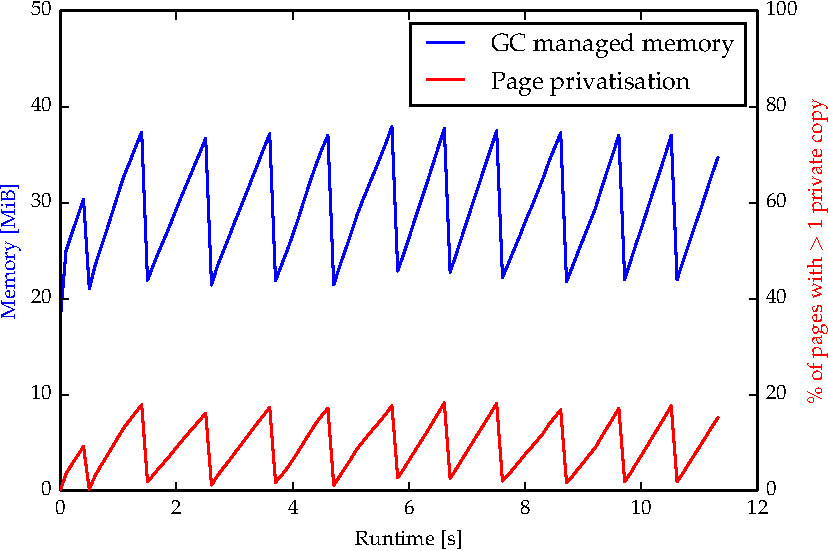
\includegraphics[width=1\columnwidth]{plots/richards_mem.pdf}
  \caption{Actual memory managed by the GC and the page privatisation
    over time in Richards benchmark\label{fig:richards_mem}}
\end{figure}



\subsection{Overhead Breakdown}

\remi{do it on a non-jit build (see reason above)}
\remi{gs:segment prefix overhead is virtually none (maybe instruction cache)}
\remi{update numbers in pypy/TODO}

\begin{itemize}
\item time taken by read \& write barriers
\item time spent committing \& aborting (maybe with different numbers
  of threads; maybe split conflict detection and obj sync on commit)
\item time in GC
\end{itemize}


\subsection{Scaling}

To asses how well the STM system scales on its own (without any real
workload), we execute the following loop on 1 to 4 threads:
\begin{lstlisting}
def workload():
    i = 20000000
    while i:
        i -= 1
\end{lstlisting}

For the results in figure \ref{fig:scaling}, we averaged
over 5 runs and normalised the average runtimes to the
time it took on a single thread. From this we see that there
is additional overhead introduced by each thread ($13\%$
for all 4 threads together).

\remi{what we don't show is by how much this overhead is influenced
by allocations}

\begin{figure}[h]
  \centering
  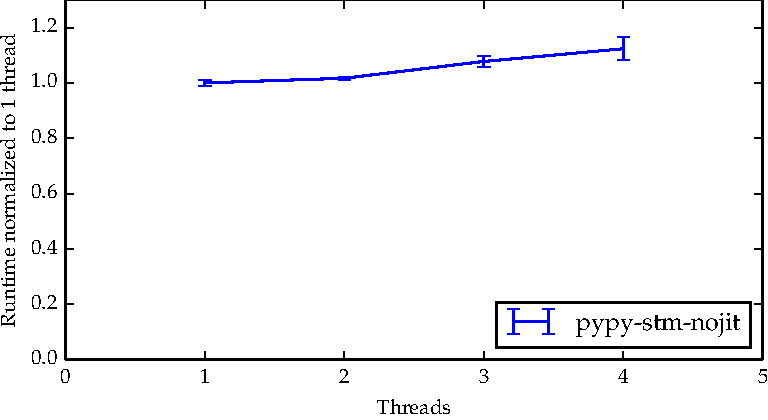
\includegraphics[width=1\columnwidth]{plots/scaling.pdf}
  \caption{Scalability of the STM system\label{fig:scaling}}
\end{figure}


\subsection{Performance Benchmarks\label{sec:performance-bench}}

\remi{For performance we first look at no-JIT behaviour of STM. Since
we cannot compete well even with CPython, we later show JIT benchmarks
where we see the unstable performance but also that we can still scale.
(with more work we can use our STM system to parallelise jitted code
too)}

more real benchmarks comparing multiple implementations:
\begin{itemize}[noitemsep]
\item pypy
\item pypy-jit
\item pypy-stm
\item pypy-stm-jit
\item cpython
\item jython
\end{itemize}


% TODO: Jython
\remi{Some benchmarks (figure \ref{fig:performance-jit} with enabled
JIT show that we can be competitive with the other solutions. It also
shows that more work is needed in that area to make performance more
stable.}

\begin{figure}[h]
  \centering
  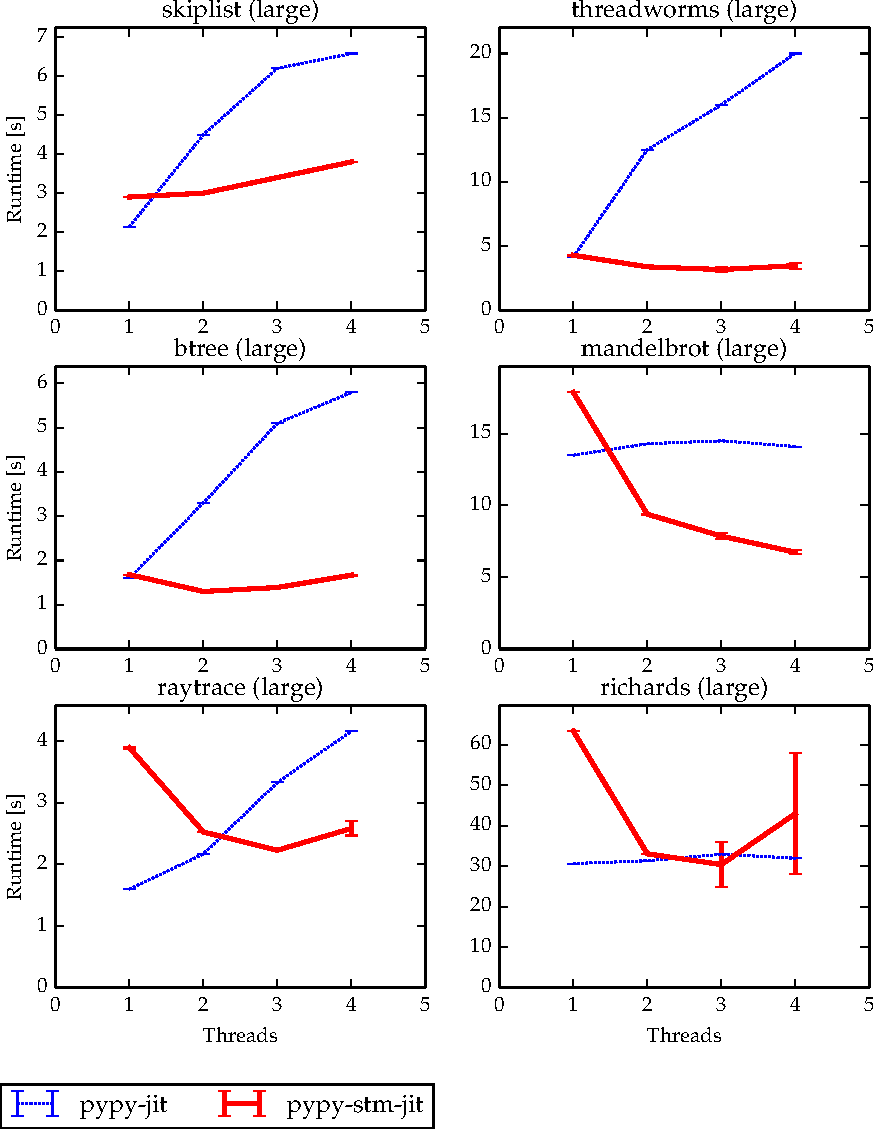
\includegraphics[width=1\columnwidth]{plots/performance.pdf}
  \caption{Comparing runtime between interpreters with JIT\label{fig:performance-jit}}
\end{figure}

\section{Related Work}


\section{Conclusions}


%% \appendix
%% \section{Appendix Title}

%% This is the text of the appendix, if you need one.

\acks
...

% We recommend abbrvnat bibliography style.

\bibliographystyle{abbrvnat}

% The bibliography should be embedded for final submission.

\begin{thebibliography}{}
\softraggedright

\bibitem{dan07}
  Dan Grossman. 2007. The transactional memory / garbage collection
  analogy. \emph{In Proceedings of the 22nd annual ACM SIGPLAN
    conference on Object-oriented programming systems and
    applications} (OOPSLA '07).

\bibitem{webjython}
  The Jython Project, \url{www.jython.org}

\bibitem{odaira14}
  Odaira, Rei, Jose G. Castanos, and Hisanobu Tomari.  "Eliminating
  global interpreter locks in Ruby through hardware transactional
  memory."  \emph{Proceedings of the 19th ACM SIGPLAN symposium on
    Principles and practice of parallel programming.} ACM, 2014.

\bibitem{warmhoff13}
  Wamhoff, Jons-Tobias, et al. "FastLane: improving performance of
  software transactional memory for low thread counts."
  \emph{Proceedings of the 18th ACM SIGPLAN symposium on Principles
    and practice of parallel programming.} ACM, 2013.

\bibitem{drago11}
  Dragojević, Aleksandar, et al. "Why STM can be more than a research
  toy." \emph{Communications of the ACM} 54.4 (2011): 70-77.

\bibitem{cascaval08}
  Cascaval, Calin, et al. "Software transactional memory: Why is it
  only a research toy?." \emph{Queue} 6.5 (2008): 40.

\bibitem{nicholas06}
  Nicholas Riley and Craig Zilles. 2006. Hardware transactional memory
  support for lightweight dynamic language evolution. \emph{In
    Companion to the 21st ACM SIGPLAN symposium on Object-oriented
    programming systems, languages, and applications} (OOPSLA
  '06). ACM, New York, NY, USA

\bibitem{fuad10}
  Fuad Tabba. 2010. Adding concurrency in python using a commercial
  processor's hardware transactional memory support. \emph{SIGARCH
  Comput. Archit. News 38}, 5 (April 2010)

\bibitem{felber07}
  Felber, Pascal, et al. "Transactifying applications using an open
  compiler framework." \emph{TRANSACT}, August (2007): 4-6.

\bibitem{bill06}
  Bill McCloskey, Feng Zhou, David Gay, and Eric
  Brewer. 2006. Autolocker: synchronization inference for atomic
  sections. \emph{In Conference record of the 33rd ACM SIGPLAN-SIGACT
  symposium on Principles of programming languages (POPL '06)}. ACM,
  New York, NY, USA

\bibitem{spear09}
  Spear, Michael F., et al. "Transactional mutex locks." \emph{SIGPLAN
    Workshop on Transactional Computing.} 2009.

\bibitem{lamport79}
  Lamport, Leslie. "How to make a multiprocessor computer that
  correctly executes multiprocess programs." \emph{Computers, IEEE
    Transactions} on 100.9 (1979): 690-691.

\bibitem{victor11}
  Victor Pankratius and Ali-Reza Adl-Tabatabai. 2011. A study of
  transactional memory vs. locks in practice. In \emph{Proceedings of
    the twenty-third annual ACM symposium on Parallelism in algorithms
    and architectures} (SPAA '11). ACM, New York, NY, USA

\bibitem{christopher10}
  Christopher J. Rossbach, Owen S. Hofmann, and Emmett
  Witchel. 2010. Is transactional programming actually
  easier?. \emph{SIGPLAN} Not. 45, 5 (January 2010), 47-56.

\bibitem{tim03}
  Tim Harris and Keir Fraser. 2003. Language support for lightweight
  transactions. \emph{In Proceedings of the 18th annual ACM SIGPLAN
    conference on Object-oriented programing, systems, languages, and
    applications} (OOPSLA '03).

\bibitem{tim05}
  Tim Harris, Simon Marlow, Simon Peyton-Jones, and Maurice
  Herlihy. 2005. Composable memory transactions. \emph{In Proceedings
    of the tenth ACM SIGPLAN symposium on Principles and practice of
    parallel programming} (PPoPP '05).

\bibitem{shan08}
  Shan Lu, Soyeon Park, Eunsoo Seo, and Yuanyuan Zhou. 2008. Learning
  from mistakes: a comprehensive study on real world concurrency bug
  characteristics. \emph{SIGARCH Comput. Archit. News} 36, 1 (March 2008),
  329-339.

\bibitem{leis14}
  Leis, Viktor, Alfons Kemper, and Thomas Neumann. "Exploiting
  Hardware Transactional Memory in Main-Memory Databases."
  \emph{Proc. of ICDE}. 2014.

\bibitem{biased}
  Kenneth Russell and David Detlefs. 2006. Eliminating
  synchronization-related atomic operations with biased locking and
  bulk rebiasing. \emph{In Proceedings of the 21st annual ACM SIGPLAN
    conference on Object-oriented programing, systems, languages, and
    applications} (OOPSLA '06).

\end{thebibliography}


\end{document}
